\title{Assignment 2.1}
\author{
        Pradyot Prakash - 130050008
            \and
        Utkarsh Mall - 130050037
			\and
		Samarth Mishra - 130260018
}
\date{\today}
\documentclass[11pt]{article}
\usepackage[left=2.5cm,top=3cm,right=2.5cm,bottom=3cm,bindingoffset=0.5cm]{geometry}
\usepackage{graphicx}
\usepackage{siunitx}
\graphicspath{ {../images/} }
\renewcommand\thesubsection{\Alph{subsection}}
\begin{document}
\maketitle

\subsection{myIntegration()}
Chosen step size $\Delta s = 1$. If a step size larger than this is chosen then information present image will missed as step size is larger than pixel size.
Choosing step size smaller than this is computationally expensive and the results of integration will be very similar to that of $\Delta s = 1$.

Bilateral interpolation is being used here. A Nearest Neighbour interpolation will not be a good estimate of integral compared to integral evaluated by bilinear interpolation.
In cases like $\Delta s = 0.66$ with integration along an axis,NN interpolation will select alternate pixels with twice, which will not be the case with bilinear interpolation.
\subsection{myRadon()}

\begin{figure}[h]
\centering
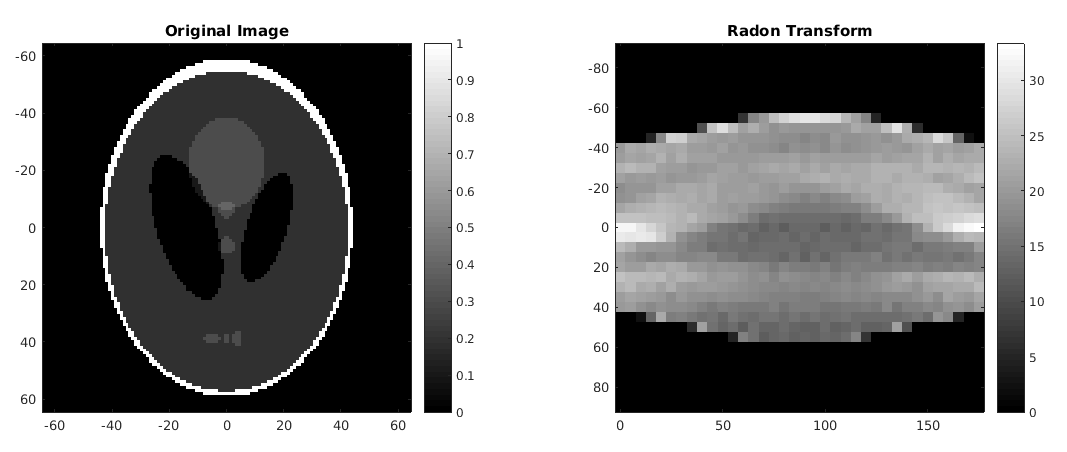
\includegraphics[scale=0.4]{b}
\caption{Shepp Logan Phantom Image and its Radon transform}
\end{figure}

\subsection{Parameter Choice}
The Radon Transform image with $\Delta s=1$ and $\Delta s=0.5$ look smoother than the transform with $\Delta s=3$. 
However there is no significant difference in images with $\Delta s=1$ and $\Delta s=0.5$.
\textbf{write reason?}

\begin{figure}[h]
\centering
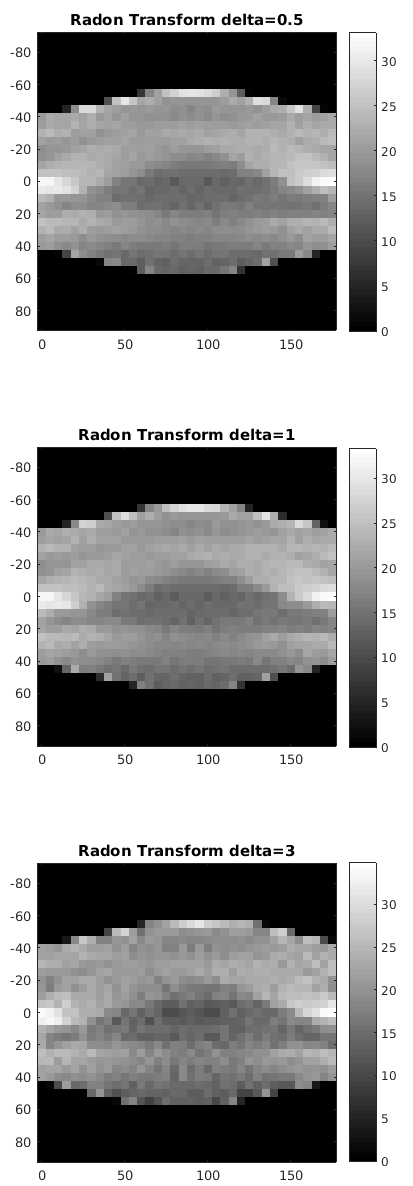
\includegraphics[scale=0.5]{c}
\caption{Shepp-Logan Phantom Image's Radon transform with $\Delta s = 0.5,1,3$ respectively}
\end{figure}
\begin{figure}[h]
\centering
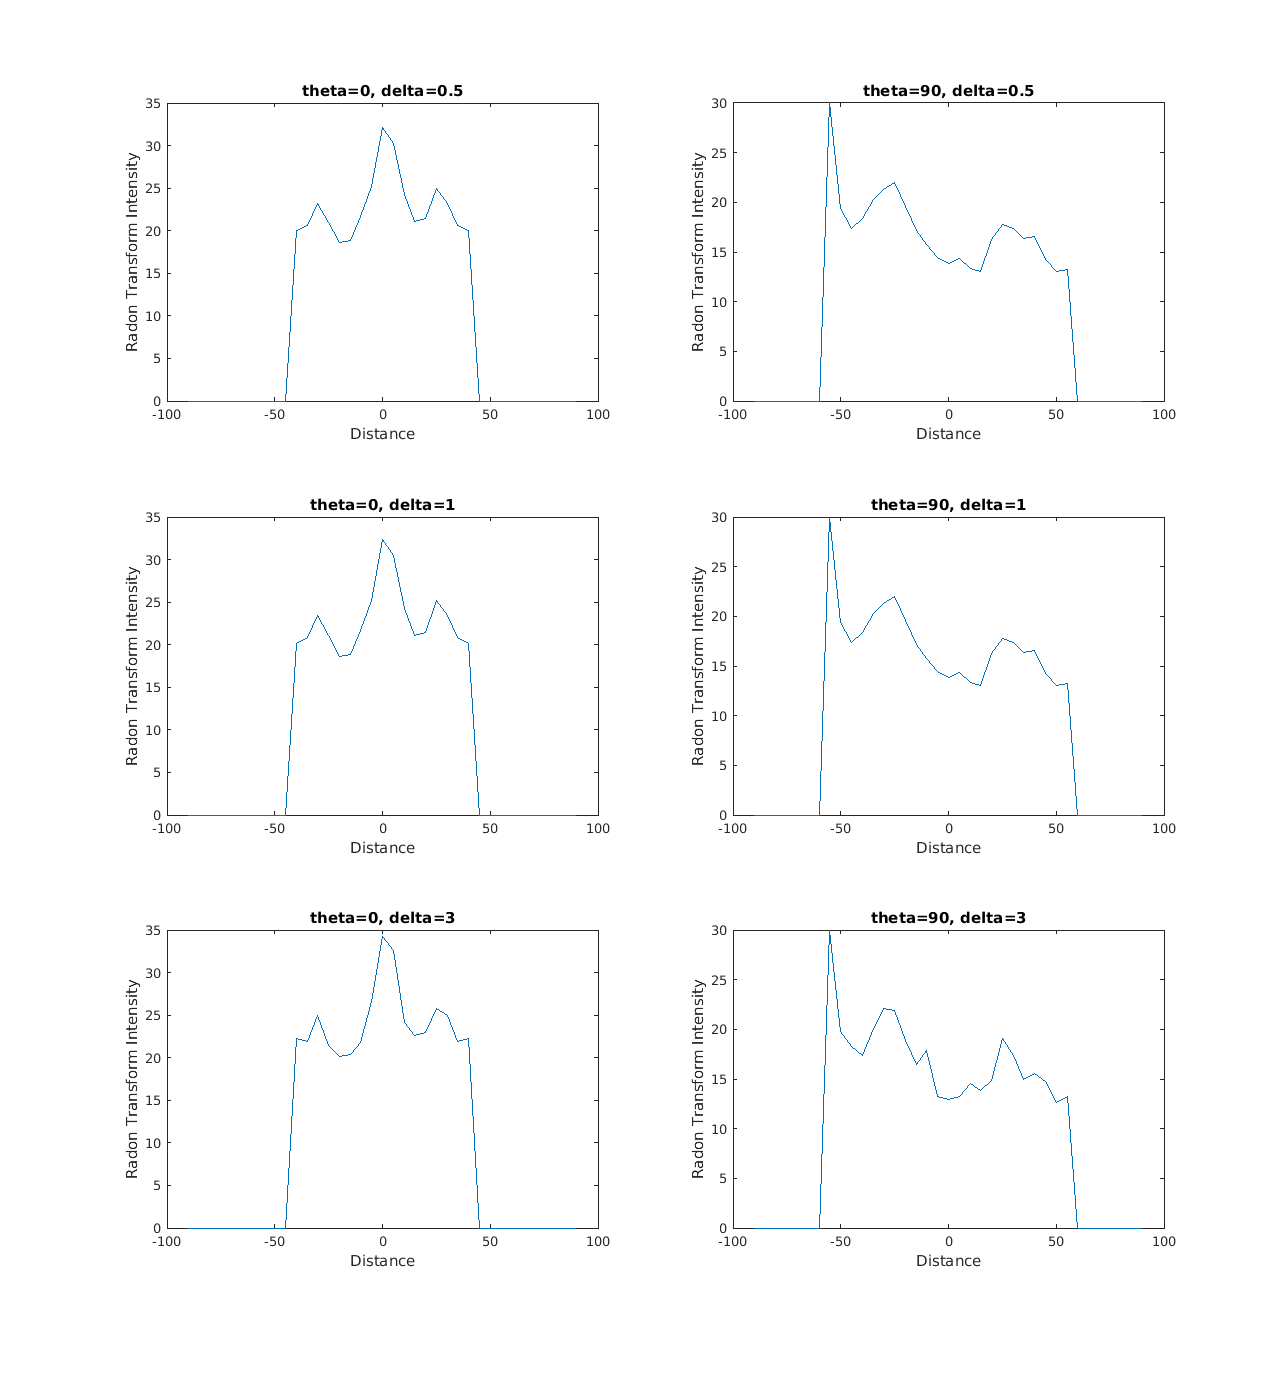
\includegraphics[scale=0.4]{c2}
\caption{Shepp-Logan Phantom Image's Radon transform Intesity along $\theta=0^{0} $ and $\theta=90^{0} $ with $\Delta s = 0.5,1,3$ respectively}
\end{figure}
The Radon Transform along a single $\theta$ with $\Delta s=1$ and $\Delta s=0.5$ are very similar and are smoother than the transform with $\Delta s=3$. 
\textbf{write reason?}

\end{document}
